% Figure from MATH 556 notes, section 36 (added, not from lecture). Compile with the notes preamble.
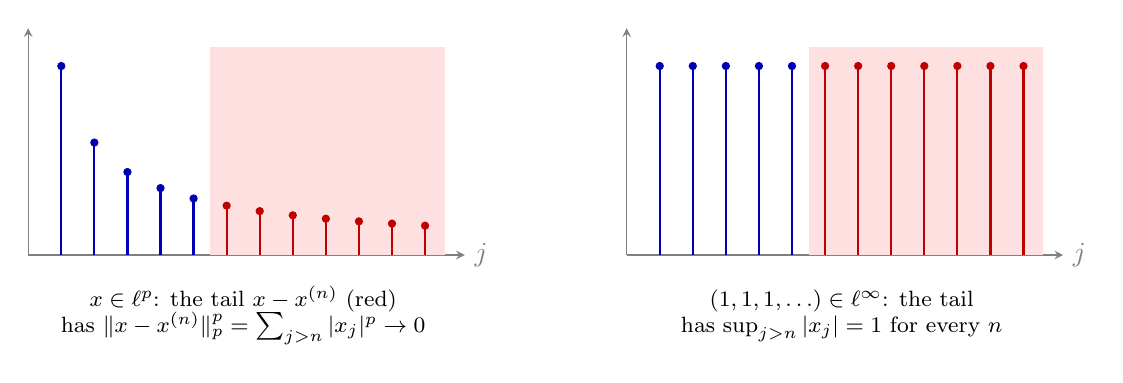
\begin{tikzpicture}[x=0.42cm, y=2.4cm, >=stealth]
  \begin{scope}
    \draw[->, gray] (0,0) -- (13.2,0) node[right] {$j$};
    \draw[->, gray] (0,0) -- (0,1.2);
    \fill[red!12] (5.5,0) rectangle (12.6,1.1);
    \draw[blue!70!black, thick] (1,0) -- (1,1); \fill[blue!70!black] (1,1) circle (1.5pt);
    \draw[blue!70!black, thick] (2,0) -- (2,0.595); \fill[blue!70!black] (2,0.595) circle (1.5pt);
    \draw[blue!70!black, thick] (3,0) -- (3,0.439); \fill[blue!70!black] (3,0.439) circle (1.5pt);
    \draw[blue!70!black, thick] (4,0) -- (4,0.354); \fill[blue!70!black] (4,0.354) circle (1.5pt);
    \draw[blue!70!black, thick] (5,0) -- (5,0.299); \fill[blue!70!black] (5,0.299) circle (1.5pt);
    \draw[red!75!black, thick] (6,0) -- (6,0.261); \fill[red!75!black] (6,0.261) circle (1.5pt);
    \draw[red!75!black, thick] (7,0) -- (7,0.232); \fill[red!75!black] (7,0.232) circle (1.5pt);
    \draw[red!75!black, thick] (8,0) -- (8,0.21); \fill[red!75!black] (8,0.21) circle (1.5pt);
    \draw[red!75!black, thick] (9,0) -- (9,0.192); \fill[red!75!black] (9,0.192) circle (1.5pt);
    \draw[red!75!black, thick] (10,0) -- (10,0.178); \fill[red!75!black] (10,0.178) circle (1.5pt);
    \draw[red!75!black, thick] (11,0) -- (11,0.166); \fill[red!75!black] (11,0.166) circle (1.5pt);
    \draw[red!75!black, thick] (12,0) -- (12,0.155); \fill[red!75!black] (12,0.155) circle (1.5pt);
    \node[font=\footnotesize, align=center] at (6.5,-0.32) {$x \in \ell^p$: the tail $x - x^{(n)}$ (red) \\ has $\|x - x^{(n)}\|_p^p = \sum_{j > n} |x_j|^p \to 0$};
  \end{scope}
  \begin{scope}[xshift=7.6cm]
    \draw[->, gray] (0,0) -- (13.2,0) node[right] {$j$};
    \draw[->, gray] (0,0) -- (0,1.2);
    \fill[red!12] (5.5,0) rectangle (12.6,1.1);
    \draw[blue!70!black, thick] (1,0) -- (1,1); \fill[blue!70!black] (1,1) circle (1.5pt);
    \draw[blue!70!black, thick] (2,0) -- (2,1); \fill[blue!70!black] (2,1) circle (1.5pt);
    \draw[blue!70!black, thick] (3,0) -- (3,1); \fill[blue!70!black] (3,1) circle (1.5pt);
    \draw[blue!70!black, thick] (4,0) -- (4,1); \fill[blue!70!black] (4,1) circle (1.5pt);
    \draw[blue!70!black, thick] (5,0) -- (5,1); \fill[blue!70!black] (5,1) circle (1.5pt);
    \draw[red!75!black, thick] (6,0) -- (6,1); \fill[red!75!black] (6,1) circle (1.5pt);
    \draw[red!75!black, thick] (7,0) -- (7,1); \fill[red!75!black] (7,1) circle (1.5pt);
    \draw[red!75!black, thick] (8,0) -- (8,1); \fill[red!75!black] (8,1) circle (1.5pt);
    \draw[red!75!black, thick] (9,0) -- (9,1); \fill[red!75!black] (9,1) circle (1.5pt);
    \draw[red!75!black, thick] (10,0) -- (10,1); \fill[red!75!black] (10,1) circle (1.5pt);
    \draw[red!75!black, thick] (11,0) -- (11,1); \fill[red!75!black] (11,1) circle (1.5pt);
    \draw[red!75!black, thick] (12,0) -- (12,1); \fill[red!75!black] (12,1) circle (1.5pt);
    \node[font=\footnotesize, align=center] at (6.5,-0.32) {$(1, 1, 1, \ldots) \in \ell^\infty$: the tail \\ has $\sup_{j > n} |x_j| = 1$ for every $n$};
  \end{scope}
\end{tikzpicture}
